\section{Time-Driven}
In the following, we derive a pure functional approach for an agent-based SIR model in which we pose solutions to the previously mentioned problems. We start out with a first approach in Yampa and show its limitations. Then we generalise it to a more powerful approach, which utilises Monadic Stream Functions, a generalisation of FRP. Finally we add a structured environment, making the example more interesting and showing the real strength of ABS over other simulation methodologies like System Dynamics and Discrete Event Simulation \footnote{The code of all steps can be accessed freely through the following URL: \url{https://github.com/thalerjonathan/phd/tree/master/public/purefunctionalepidemics/code}}.

\subsection{The SIR model}
The \textit{explanatory} SIR model is a very well studied and understood compartment model from epidemiology \cite{kermack_contribution_1927}, which allows to simulate the dynamics of an infectious disease like influenza, tuberculosis, chicken pox, rubella and measles spreading through a population.

In this model, people in a population of size $N$ can be in either one of three states \textit{Susceptible}, \textit{Infected} or \textit{Recovered} at a particular time, where it is assumed that initially there is at least one infected person in the population. People interact \textit{on average} with a given rate of $\beta$ other people per time-unit and become infected with a given probability $\gamma$ when interacting with an infected person. When infected, a person recovers \textit{on average} after $\delta$ time-units and is then immune to further infections. An interaction between infected persons does not lead to re-infection, thus these interactions are ignored in this model. This definition gives rise to three compartments with the transitions seen in Figure \ref{fig:sir_transitions}.

\begin{figure}
	\centering
	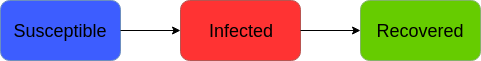
\includegraphics[width=.4\textwidth, angle=0]{./fig/fpabs/timedriven/SIR_transitions.png}
	\caption{States and transitions in the SIR compartment model.}
	\label{fig:sir_transitions}
\end{figure}

This model was also formalized using System Dynamics (SD) \cite{porter_industrial_1962}. In SD one models a system through differential equations, allowing to conveniently express continuous systems, which change over time, solving them by numerically integrating over time, which gives then rise to the dynamics. The SIR model is modelled using the following equation, with the dynamics shown in Figure \ref{fig:sir_sd_dynamics} .

\begin{equation}
\begin{aligned}
\frac{\mathrm d S}{\mathrm d t} = -infectionRate \\
\frac{\mathrm d I}{\mathrm d t} = infectionRate - recoveryRate \\
\frac{\mathrm d R}{\mathrm d t} = recoveryRate 
\end{aligned}
\end{equation}

\begin{equation}
\begin{aligned}
infectionRate = \frac{I \beta S \gamma}{N} \\
recoveryRate = \frac{I}{\delta} 
\end{aligned}
\end{equation}

\begin{figure}
	\centering
	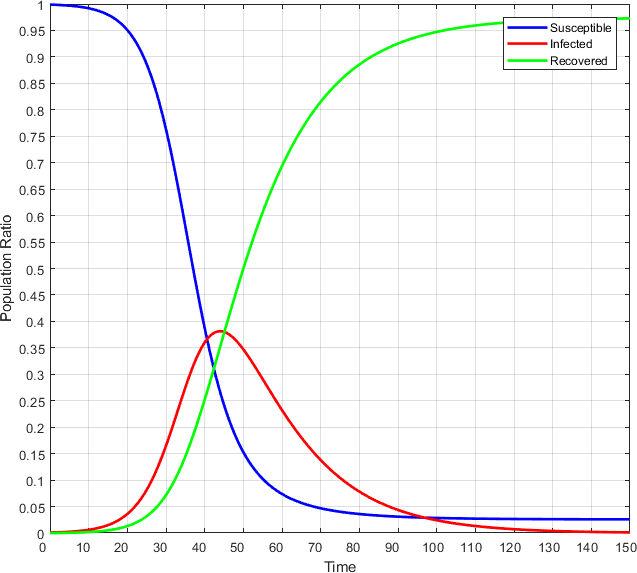
\includegraphics[width=0.5\textwidth, angle=0]{./fig/fpabs/timedriven/SIR_SD_1000agents_150t_001dt.png}
	\caption{Dynamics of the SIR compartment model using the System Dynamics approach. Population Size $N$ = 1,000, contact rate $\beta =  \frac{1}{5}$, infection probability $\gamma = 0.05$, illness duration $\delta = 15$ with initially 1 infected agent. Simulation run for 150 time-steps. Generated using our pure functional SD approach (see Chapter \ref{sub:generalising_system_dynamics}).}
	\label{fig:sir_sd_dynamics}
\end{figure}

The approach of mapping the SIR model to an ABS is to discretize the population and model each person in the population as an individual agent. The transitions between the states are happening due to discrete events caused both by interactions amongst the agents and time-outs. The major advantage of ABS is that it allows to incorporate spatiality as shown in Section \ref{sec:adding_env} and simulate heterogenity of population e.g. different sex, age. This is not possible with other simulation methods e.g. SD or Discrete Event Simulation \cite{zeigler_theory_2000}.

According to the model, every agent makes \textit{on average} contact with $\beta$ random other agents per time unit. In ABS we can only contact discrete agents thus we model this by generating a random event on average every $\frac{1}{\beta}$ time units. We need to sample from an exponential distribution because the rate is proportional to the size of the population \cite{borshchev_system_2004}. Note that an agent does not know the other agents' state when making contact with it, thus we need a mechanism in which agents reveal their state in which they are in \textit{at the moment of making contact}. This mechanism is an implementation detail, which we will derive in our implementation steps. For now we only assume that agents can make contact with each other somehow.

The \textit{parallel} strategy matches the semantics of the agent-based SIR model due to the underlying roots in the System Dynamics approach. As discussed already in Chapter \ref{sub:par_strategy}, in the parallel update-strategy, the agents act conceptually all at the same time in lock-step. This implies that they observe the same environment state during a time-step and actions of an agent
are only visible in the next time-step - they are isolated from each other. As will become apparent, FP can be used to enforce the correct application of this strategy already on the compile-time level.

\subsection{A pure functional implementation}
TODO: follow the PFE paper but add a few references back to the implementing ABS chapter so it is clear what problems we are currently solving. also might explain some concepts bit more in depth e.g. continuations?

As described in the Chapter \ref{sec:back_frp}, Arrowized FRP \cite{hughes_generalising_2000} is a way to implement systems  with continuous and discrete time-semantics where the central concept is the signal function, which can be understood as a process over time, mapping an input- to an output-signal. Technically speaking, a signal function is a continuation which allows to capture state using closures and hides away the $\Delta t$, which means that it is never exposed explicitly to the programmer, meaning it cannot be manipulated.

As already pointed out, agents need to perceive time, which means that the concept of processes over time is an ideal match for our agents and our system as a whole, thus we will implement them and the whole system as signal functions.

\subsection{Discussion}
Our FRP based approach is different from traditional approaches in the ABS community. First it builds on the already quite powerful FRP paradigm. Second, due to our continuous time approach, it forces one to think properly of time-semantics of the model and how small $\Delta t$ should be. Third it requires one to think about agent interactions in a new way instead of being just method-calls.

Because no part of the simulation runs in the IO Monad and we do not use \textit{unsafePerformIO} we can rule out a serious class of bugs caused by implicit data-dependencies and side-effects, which can occur in traditional imperative implementations.

Also we can statically guarantee the reproducibility of the simulation, which means that repeated runs with the same initial conditions are guaranteed to result in the same dynamics. Although we allow side-effects within agents, we restrict them to only the Random Monad in a controlled, deterministic way and never use the IO Monad, which guarantees the absence of non-deterministic side effects within the agents and other parts of the simulation.

Determinism is also ensured by fixing the $\Delta t$ and not making it dependent on the performance of e.g. a rendering-loop or other system-dependent sources of non-determinism as described by \cite{perez_testing_2017}. Also by using FRP we gain all the benefits from it and can use research on testing, debugging and exploring FRP systems \cite{perez_testing_2017, perez_back_2017}.

Also we showed how to implement the \textit{parallel} update-strategy \cite{thaler_art_2017} in a way that the correct semantics are enforced and guaranteed already at compile time through the types. This is not possible in traditional imperative implementations and poses another unique benefit over the use of functional programming in ABS.

The result of using FRP allows expressing continuous time-semantics in a very clear, compositional and declarative way, abstracting away the low-level details of time-stepping and progress of time within an agent.
	
Our approach can guarantee reproducibility already at compile time, which means that repeated runs of the simulation with the same initial conditions will always result in the same dynamics, something highly desirable in simulation in general. This can only be achieved through purity, which guarantees the absence of implicit side-effects, which allows to rule out non-deterministic influences at compile time through the strong static type system, something not possible with traditional object-oriented approaches. Further, through purity and the strong static type system, we can rule out important classes of run-time bugs e.g. related to dynamic typing, and the lack of implicit data-dependencies which are common in traditional imperative object-oriented approaches.
	
Using pure functional programming, we can enforce the correct semantics of agent execution through types where we demonstrate that this allows us to have both, sequential monadic behaviour, and agents acting \textit{conceptually} at the same time in lock-step, something not possible using traditional object-oriented approaches.

Currently, the performance of the system does not come close to imperative implementations. We compared the performance of our pure functional approach as presented in Section \ref{sec:adding_env} to an implementation in Java using the ABS library RePast \cite{north_complex_2013}. We ran the simulation until $t = 100$ on a 51x51 (2,601 agents) with $\Delta t = 0.1$ (unknown in RePast) and averaged 8 runs. The performance results make the lack of speed of our approach quite clear: the pure functional approach needs around 72.5 seconds whereas the Java RePast version just 10.8 seconds on our machine to arrive at $t = 100$. It must be mentioned, that RePast does implement an event-driven approach to ABS, which can be much more performant \cite{meyer_event-driven_2014} than a time-driven one as ours, so the comparison is not completely valid. Still, we have already started investigating speeding up performance through the use of Software Transactional Memory \cite{harris_composable_2005, harris_transactional_2006}, which is quite straight forward when using MSFs. It shows very good results but we have to leave the investigation and optimization of the performance aspect of our approach for further research as it is beyond the scope of this paper.

Despite the strengths and benefits we get by leveraging on FRP, there are errors that are not raised at compile time, e.g. we can still have infinite loops and run-time errors. This was for example investigated in \cite{sculthorpe_safe_2009} where the authors use dependent types to avoid some run-time errors in FRP. We suggest that one could go further and develop a domain specific type system for FRP that makes the FRP based ABS more predictable and that would support further mathematical analysis of its properties. Furthermore, moving to dependent types would pose a unique benefit over the traditional object-oriented approach and should allow us to express and guarantee even more properties at compile time. We leave this for further research.

In our pure functional approach, agent identity is not as clear as in traditional object-oriented programming, where there is a quite clear concept of object-identity through the encapsulation of data and methods. Signal functions don't offer this strong identity and one needs to build additional identity mechanisms on top e.g. when sending messages to specific agents.

We can conclude that the main difficulty of a pure functional approach evolves around the communication and interaction between agents, which is a direct consequence of the issue with agent identity. Agent interaction is straight-forward in object-oriented programming, where it is achieved using method-calls mutating the internal state of the agent, but that comes at the cost of a new class of bugs due to implicit data flow. In pure functional programming these data flows are explicit but our current approach of feeding back the states of all agents as inputs is not very general. We have added further mechanisms of agent interaction which we had to omit due to lack of space.

\subsection{Other approaches}
Sequential: see event-driven
Concurrent: see STM chapter
Actor: not discussed in this thesis but briefly 

\subsection{Super-Sampling}
when super-sampling is mentioned in the PFE paper extend it and add FrABS report, also show superSampling function implementation from PFE paper and FrABS with full body implementation